\documentclass[english,man]{apa6}

\usepackage{amssymb,amsmath}
\usepackage{ifxetex,ifluatex}
\usepackage{fixltx2e} % provides \textsubscript
\ifnum 0\ifxetex 1\fi\ifluatex 1\fi=0 % if pdftex
  \usepackage[T1]{fontenc}
  \usepackage[utf8]{inputenc}
\else % if luatex or xelatex
  \ifxetex
    \usepackage{mathspec}
    \usepackage{xltxtra,xunicode}
  \else
    \usepackage{fontspec}
  \fi
  \defaultfontfeatures{Mapping=tex-text,Scale=MatchLowercase}
  \newcommand{\euro}{€}
\fi
% use upquote if available, for straight quotes in verbatim environments
\IfFileExists{upquote.sty}{\usepackage{upquote}}{}
% use microtype if available
\IfFileExists{microtype.sty}{\usepackage{microtype}}{}

% Table formatting
\usepackage{longtable, booktabs}
\usepackage{lscape}
% \usepackage[counterclockwise]{rotating}   % Landscape page setup for large tables
\usepackage{multirow}		% Table styling
\usepackage{tabularx}		% Control Column width
\usepackage[flushleft]{threeparttable}	% Allows for three part tables with a specified notes section
\usepackage{threeparttablex}            % Lets threeparttable work with longtable

% Create new environments so endfloat can handle them
% \newenvironment{ltable}
%   {\begin{landscape}\begin{center}\begin{threeparttable}}
%   {\end{threeparttable}\end{center}\end{landscape}}

\newenvironment{lltable}
  {\begin{landscape}\begin{center}\begin{ThreePartTable}}
  {\end{ThreePartTable}\end{center}\end{landscape}}

  \usepackage{ifthen} % Only add declarations when endfloat package is loaded
  \ifthenelse{\equal{\string man}{\string man}}{%
   \DeclareDelayedFloatFlavor{ThreePartTable}{table} % Make endfloat play with longtable
   % \DeclareDelayedFloatFlavor{ltable}{table} % Make endfloat play with lscape
   \DeclareDelayedFloatFlavor{lltable}{table} % Make endfloat play with lscape & longtable
  }{}%



% The following enables adjusting longtable caption width to table width
% Solution found at http://golatex.de/longtable-mit-caption-so-breit-wie-die-tabelle-t15767.html
\makeatletter
\newcommand\LastLTentrywidth{1em}
\newlength\longtablewidth
\setlength{\longtablewidth}{1in}
\newcommand\getlongtablewidth{%
 \begingroup
  \ifcsname LT@\roman{LT@tables}\endcsname
  \global\longtablewidth=0pt
  \renewcommand\LT@entry[2]{\global\advance\longtablewidth by ##2\relax\gdef\LastLTentrywidth{##2}}%
  \@nameuse{LT@\roman{LT@tables}}%
  \fi
\endgroup}


  \usepackage{graphicx}
  \makeatletter
  \def\maxwidth{\ifdim\Gin@nat@width>\linewidth\linewidth\else\Gin@nat@width\fi}
  \def\maxheight{\ifdim\Gin@nat@height>\textheight\textheight\else\Gin@nat@height\fi}
  \makeatother
  % Scale images if necessary, so that they will not overflow the page
  % margins by default, and it is still possible to overwrite the defaults
  % using explicit options in \includegraphics[width, height, ...]{}
  \setkeys{Gin}{width=\maxwidth,height=\maxheight,keepaspectratio}
\ifxetex
  \usepackage[setpagesize=false, % page size defined by xetex
              unicode=false, % unicode breaks when used with xetex
              xetex]{hyperref}
\else
  \usepackage[unicode=true]{hyperref}
\fi
\hypersetup{breaklinks=true,
            pdfauthor={},
            pdftitle={Methods to Detect Low Quality Data and Its Implication for Psychological Research},
            colorlinks=true,
            citecolor=blue,
            urlcolor=blue,
            linkcolor=black,
            pdfborder={0 0 0}}
\urlstyle{same}  % don't use monospace font for urls

\setlength{\parindent}{0pt}
%\setlength{\parskip}{0pt plus 0pt minus 0pt}

\setlength{\emergencystretch}{3em}  % prevent overfull lines

\ifxetex
  \usepackage{polyglossia}
  \setmainlanguage{}
\else
  \usepackage[english]{babel}
\fi

% Manuscript styling
\captionsetup{font=singlespacing,justification=justified}
\usepackage{csquotes}
\usepackage{upgreek}

 % Line numbering
  \usepackage{lineno}
  \linenumbers


\usepackage{tikz} % Variable definition to generate author note

% fix for \tightlist problem in pandoc 1.14
\providecommand{\tightlist}{%
  \setlength{\itemsep}{0pt}\setlength{\parskip}{0pt}}

% Essential manuscript parts
  \title{Methods to Detect Low Quality Data and Its Implication for Psychological
Research}

  \shorttitle{Detection Methods}


  \author{Erin M. Buchanan\textsuperscript{1}~\& John E. Scofield\textsuperscript{2}}

  % \def\affdep{{"", ""}}%
  % \def\affcity{{"", ""}}%

  \affiliation{
    \vspace{0.5cm}
          \textsuperscript{1} Missouri State University\\
          \textsuperscript{2} University of Missouri  }

  \authornote{
    Erin M. Buchanan, Department of Psychology, Missouri State University;
    John E. Scofield, Department of Psychological Sciences, University of
    Missouri.
    
    Correspondence concerning this article should be addressed to Erin M.
    Buchanan, 901 S. National Ave, Springfield, MO, 65804. E-mail:
    \href{mailto:erinbuchanan@missouristate.edu}{\nolinkurl{erinbuchanan@missouristate.edu}}
  }


  \abstract{Web-based data collection methods such as Amazon's Mechanical Turk (AMT)
are an appealing option to recruit participants quickly and cheaply for
psychological research. While concerns regarding data quality have
emerged with AMT, several studies have exhibited that data collected via
AMT are as reliable as traditional college samples and are often more
diverse and representative of noncollege populations. The development of
methods to screen for low quality data, however, has been less explored.
Omitting participants based on simple screening methods in isolation,
such as response time or attention checks may not be adequate
identification methods, with an inability to delineate between high or
low effort participants. Additionally, problematic survey responses may
arise from survey automation techniques such as survey bots or automated
form fillers. The current project developed low quality data detection
methods while overcoming previous screening limitations. Multiple checks
were employed, such as page response times, distribution of survey
responses, the number of utilized choices from a given range of scale
options, click counts, and manipulation checks. This method was tested
on a survey taken with an easily available plug-in survey bot, as well
as compared to data collected by human participants providing both high
effort and randomized, or low effort, answers. Identified cases can then
be used as part of sensitivity analyses to warrant exclusion from
further analyses. This algorithm can be a promising tool to identify low
quality or automated data via AMT or other online data collection
platforms.}
  \keywords{Amazon Mechanical Turk, survey automation, participant screening, data
quality \\

    
  }





\usepackage{amsthm}
\newtheorem{theorem}{Theorem}
\newtheorem{lemma}{Lemma}
\theoremstyle{definition}
\newtheorem{definition}{Definition}
\newtheorem{corollary}{Corollary}
\newtheorem{proposition}{Proposition}
\theoremstyle{definition}
\newtheorem{example}{Example}
\theoremstyle{definition}
\newtheorem{exercise}{Exercise}
\theoremstyle{remark}
\newtheorem*{remark}{Remark}
\newtheorem*{solution}{Solution}
\begin{document}

\maketitle

\setcounter{secnumdepth}{0}



Amazon Mechanical Turk (AMT) was created in 2005 to serve as a
marketplace where tasks and miscellaneous jobs are performed by
\enquote{workers} in exchange for monetary compensation. Tasks range in
size and time commitment, where payment for tasks are usually a function
of the time commitment. Workers are able to complete tasks remotely
around the world, so demographic makeup is naturally more representative
compared to traditional WEIRD (Western, Educated, Industrialized, Rich,
Democratic) subject pools (Henrich, Heine, \& Norenzayan, 2010).
Typically, about half of workers come from within the United States,
whereas upwards to 40\% of workers can come from India (Ipeirotis,
2010). Slightly more females than males have also been documented as AMT
workers (Paolacci, Chandler, \& Ipeirotis, 2010).

With a large pool of workers available at any given time, AMT is an
extremely attractive market for researchers posting studies or
experiments, especially with the prospect that data collection from
studies can be completed quickly and cheaply (Chandler \& Paolacci,
2017; Downs, Holbrook, Sheng, \& Cranor, 2010; Mason \& Suri, 2012).
Tasks posted from researchers can range between writing tasks,
traditional surveys, or even participating in experiments. Since 2005,
AMT has quickly become a popular and accessible tool for researchers,
especially in the social sciences (Buhrmester, Kwang, \& Gosling, 2011).
This popularity has been reflected in academic literature, as over 500
articles in 2015 alone reported utilizing AMT as a means to collect data
(Chandler \& Paolacci, 2017). Notably, those aforementioned articles
were published in academic journals with an impact factor exceeding 2.5
(Chandler \& Paolacci, 2017), suggesting community acceptance of the use
of AMT as a viable subject pool.

Although the use of AMT as a subject pool has undoubtedly become an
invaluable tool for researchers with limited time or budgets, concerns
still arise regarding the pay structure for workers. Downs et al. (2010)
elucidates that payments are suggested to reflect a reasonable rate,
with eight dollars per hour being a reasonable minimum (13 cents per
minute). However, feedback from actual AMT workers indicated that a fair
price included a range as low as around \$3.50 per hour (Sorokin \&
Forsyth, 2008). Small monetary payouts can be considered a question of
research ethics (Fort, Adda, \& Cohen, 2011), and Felstiner (2011)
further discusses the debate and ethical implications of compensation
for crowd-source platforms such as AMT. Small monetary compensation for
workers also brings up questions regarding whether subjects take tasks
at hand in a serious matter or with complete attention (Downs et al.,
2010; Paolacci et al., 2010). This point can be especially plausible
considering the anonymous nature of many research experiments. However,
Mason and Suri (2012) found that financial compensation was not
typically a main motivating factor when completing tasks, and that a
good majority of participants considered the quality of work they were
providing. Moreover, from a quality check perspective, data quality were
found to be invariant to changes in the level of pay workers receive for
various tasks (Buhrmester et al., 2011).

\subsection{Quality of Data}\label{quality-of-data}

Apart from concerns about worker payment, questions have surfaced about
the quality of data researchers obtain from crowd-sourcing platforms
like AMT. One initial concern centers on how representative subject
samples are compared to traditional subject pools, like at colleges and
universities. Previous research has shown that participants recruited
via AMT are at a minimum as representative as traditional participant
pools. In many cases participants are more representative and closer to
a general population in geographical location and age (Berinsky, Huber,
\& Lenz, 2012; Casler, Bickel, \& Hackett, 2013; Paolacci \& Chandler,
2014; Paolacci et al., 2010). In some cases utilizing these online
platforms can be beneficial, overcoming inherent limitations from
certain WEIRD participant pools from colleges and universities.

In addition to representative samples matching or exceeding standards
set by traditional subject pools, there is a paucity of research to
indicate that the quality of data provided by AMT workers is any worse
than college samples. Crowd-sourcing platform data from multiple studies
were found to be nearly tantamount to traditional sampling (Gosling,
Vazire, Srivastava, \& John, 2004; Krantz \& Dalal, 2000). Paolacci et
al. (2010) found AMT to be a reliable source to collect experimental
data in judgment and decision-making paradigms, and a slew of other
comparisons between traditional sampling and online data collection with
multiple types of experimental tasks have generally found similar
reliability (Goodman, Cryder, \& Cheema, 2012; Gosling et al., 2004;
Mason \& Suri, 2012; Suri, Goldstein, \& Mason, 2011). Overall,
Buhrmester et al. (2011) concluded that data collected from AMT
sufficiently meets common psychometric standards that are prevalent in
the academic literature. Using online methods for data collection can
additionally help to mitigate other confounding concerns, such as
experimenter bias or participant reactance, which can be problematic in
laboratory and in person experimental settings. An attenuation of these
potentially limiting biases can help the internal validity associated
with experiments run through AMT (Paolacci et al., 2010).

\subsection{Data Screening Methods}\label{data-screening-methods}

A serious concern with any data provided by human participants is the
quality of the data, as the standard of garbage in, garbage out applies
to any form of statistical analysis. There are multiple ways in which
data can be screened to help increase the quality of data, while
mitigating various forms of noise. One such method would be to examine
the length of time participants spent on a given task. By indicating
which participants spent an implausibly short amount of time on a task,
we may be able to eliminate inappropriate data (i.e., random clicks by
participants). Downs et al. (2010) examined time and its effects on
performance by setting a threshold at the 90th percentile for time spent
on a given task as valid data. Performance, however, was not remarkably
better between participants who did and did not finish quickly, and so
Downs et al. (2010) suggested that setting thresholds may not be an
adequate identifier for those who are, so to speak, \enquote{gaming the
system}. Goodman et al. (2012) also noted that when analyzing
differences in task performance, the fastest 8\% did not do much better
than the rest of the sample and the fastest 3\% of respondents only did
slightly worse compared to the rest of the sample. However, Mason and
Suri (2012) suggested that using the time spent completing a certain
task can be a viable way of screening out low effort responses.

Stieger and Reips (2010) developed an innovative tool
(UserActionTracer), allowing researchers to collect more behavioral
information that otherwise would be difficult to ascertain using
existing survey software. Simple JavaScript code was implemented
alongside online surveys, enabling the collection of various metrics
such as the frequency of unfilled items, frequency of changed answers,
mouse click rates, and excessive mouse movements. By identifying
abnormal occurrences of these metrics, Stieger and Reips (2010) were
able to indicate participants with potential low motivation, which could
lead to low data quality. \enquote{Clicking through}, or responding to
questions at a rate faster than the average reading time of a given
question was found to be the most common occurrence. These types of
tools have practical importance not only in the detection of potentially
low quality data, but can be used in the future development of
questionnaires in terms of participant usability.

Another method includes the use of attention checks or gold standard
questions. These are questions with obvious answers, such as
\enquote{Please choose the second option for this question}, as a means
of assessing active participation among participants. Paolacci et al.
(2010) advocates for the use of attention checks to help screen for
attentiveness. However, Goodman et al. (2012) stated concerns regarding
the exclusion of participants from response times or attention checks
alone. These concerns revolve around potentially biasing samples.
Researchers could additionally ask pre-screening questions in attempts
to test participants of a certain nature. By employing logic in many
online surveys, participants can be routed to an end of a survey if
certain answers (e.g., demographic information) are not selected in a
survey. Current screening methods still vary depending on the nature of
the present task. With mixed results regarding the use of certain types
of screening methods, a better aim is to develop more reliable methods
for screening participants.

\subsection{Purpose of Current Study}\label{purpose-of-current-study}

Fraudulent participant responses can be problematic for any study,
leading to the question of appropriate screening methods. Chandler and
Paolacci (2017) found that AMT workers wished more work was available to
them, which in turn may influence motivations to lie about
characteristics, or find means to provide fraudulent responses (Berg,
Lindeboom, \& Dolton, 2006). Participants may use tactics such as
reloading surveys and changing previous answers if a pre-screening
question has become apparent. While many online platforms, such as
Qualtrics, have options to prevent duplicate responses (i.e., ballot
stuffing), duplicate responses can still be possible. Chandler and
Paolacci (2017) found evidence that even after utilizing options to
prevent duplicate responses, 3\% of responses were found to be
duplicates. An alternate form of suspicious survey responses stem not
from human participants, but from survey automation techniques such as
survey bots or automated form fillers. Automated form fillers allow
participants to complete entire surveys with one or two clicks. For
instance, certain browser plug-ins randomly select radio buttons among
common types of survey responses (e.g., Likert style questions).
Similarly, when able to overcome constraints such as preventative
methods to curtail ballot stuffing, survey bots could be a method to
efficiently complete the same survey multiple times.

The current project investigated this question in two studies. Overall,
Study 1 examined methods of data completion to develop an algorithm to
detect low quality responses. In Study 1a, we investigated the
characteristics of automated form fillers on Likert style data and used
those characteristics to help develop automation detection methods. In
Study 1b, we explored data quality by examining the differences between
automated, high effort, and low effort participant responses to refine
the algorithm. Study 2 was used to investigate the rate of automated and
low effort responses in a given sample of AMT workers. Sensitivity
analyses were then used to compare differences in responses given
various ratios of high effort to low effort/automated responses. This
study was pre-registered at the Open Science Framework
(\url{https://osf.io/erqzm/}), and all materials, data, and R code are
available at \url{https://osf.io/x6t8a/}.

\section{Study 1a - Automated Form
Fillers}\label{study-1a---automated-form-fillers}

\section{Method}\label{method}

\subsection{Simulated Data}\label{simulated-data}

To investigate the possibility of automated survey responses, a survey
bot was constructed to investigate characteristics of survey responses
completed by automated form fillers. The survey bot was created using
the \enquote{Form Filler} Google Chrome plug-in, which automatically
inputs all selection within a given page with dummy data. This plugin
was used in both the algorithm development, as well as Study 1b
participant testing. The survey bot was constructed using Python, which
navigated to an online survey, simulating mouse movements and clicks in
an iterative fashion. The survey bot imputed and submitted random
values, iterated over one thousand times until complete data was
available for 1000 rows. The online survey simply consisted of 100
Likert style questions with a scale range from one to seven. Since this
data was created with the automated filler, no real questions or scale
values were used (i.e., an empty shell of a survey was created for this
part of the project). Scale values, along with page response times and
click counts were extracted from the Qualtrics database with an aim to
generally explore the characteristics of automated survey responses.

\section{Results}\label{results}

\subsection{Click Count}\label{click-count}

The click count was operationalized as the total number of times that a
participant clicked on the survey page. Ideally, this number has a
minimum of the number of questions on that page. For instance, if a
survey has 15 questions, we should expect a minimum of 15 clicks for an
active human participant who has answered every question. The page
submit button (i.e., continue, next, submit) does not record a click. In
this data, click count is zero with no variance, as Qualtrics does not
always register clicks from automated form fillers.

\subsection{Page Timing}\label{page-timing}

Qualtrics often provides different measures of timing, including the
time it takes for the first and last click, and the submission of the
survey page, all beginning from when the page first loaded. We found
that the time to first click and last click were zero, as no clicks were
recorded. The page submit time averaged \emph{M} = 3.56 seconds
(\emph{SD} = 0.23). The lower quantile of the page submit time was 3.34
seconds and the upper quantile was 3.79 seconds. Each individual page of
a survey gives the researcher the ability to see what data might be
usable by examining each set of questions for page submit times and
click count. Additionally, depending on the programming of the original
survey, participants may be able to close out of survey and return at a
later date to finish. This survey setup can result in a total survey
duration time of several days, making total survey duration an
unreliably difficult metric to judge for low effort responses.

\subsection{Data Distribution}\label{data-distribution}

A histogram was used to examine the pattern of responses provided by the
survey bot. The responses to the blank questions on the survey were
examined across all rows, and, as expected, the data were uniform across
the seven Likert scale options. The average skew for responses was less
than 0.01 (\emph{SD} = 0.14) and the average kurtosis was 1.77
(\emph{SD} = 0.11).

\section{Study 1b - Participant Data
Quality}\label{study-1b---participant-data-quality}

\section{Method}\label{method-1}

\subsection{Participants}\label{participants}

Next, survey response characteristics were compared between different
means of survey completion by participants. The survey was first sent to
the research team of the investigators, and then the investigator's
summer undergraduate and graduate courses. Additional participants were
recruited the first week of data collection in the fall semester from
the undergraduate participant pool at a large Midwestern university. We
originally aimed for a sample size of \emph{N} = 100, and preemptively
recruited more participants to allow for the exclusion of incorrect
responses (i.e., participants who did not fill out the survey
correctly). The overall dataset initially included 202 participants. 16
participants were excluded for failing to consent to the study. 64
participants were excluded for failing to complete the study 100\%. As
described below, we employed attention checks to ensure that our test
data was appropriate, and 14 more participants were excluded due to
incorrect answers on the manipulation checks. Last, we excluded
participants who used the survey automation on the incorrect section, as
determined by click counts, and another 14 were excluded. Therefore,
final \emph{N} for the study was 94. Participants were given course
credit for their participation.

\subsection{Materials}\label{materials}

The survey used was the Resilience Scale 14 Items (RS-14) which measures
an individual's resiliency through items covering meaning/purpose,
perseverance, equanimity, self-reliance, and existential loneliness
(Wagnild, 2009; Wagnild \& Young, 1993). This scale uses a 1
(\emph{strongly disagree}) to 7 (\emph{strongly agree}) Likert response
scale. Survey questions can be found at www.resiliencecenter.com to find
specific RS-14 item content. This questionnaire has been previously
investigated by the investigators (Aiena, Baczwaski, Schulenberg, \&
Buchanan, 2014) across clinical and undergraduate samples and was found
to be reliable and valid. Real questionnaire questions were used in
order to examine reading times and authentic answers. An additional item
manipulation check was embedded into each page of the survey that read:
\enquote{Please mark strongly agree for this question.} The complete
survey can be found in the online supplementary materials at
\url{https://osf.io/x6t8a/}.

\subsection{Design and Procedure}\label{design-and-procedure}

Participants were routed to an online Qualtrics survey. The same survey
was completed three times in a randomized order, thus, the study used a
repeated measures design. The first condition was active participation,
where subjects were instructed to truthfully and actively complete the
survey by reading and answering each question. The second condition was
the random, or low effort condition, where participants were instructed
not to read the questions but to merely select random answers at their
own pace to complete the survey. The third and final condition was the
automated response condition, in which participants were instructed to
complete the survey using an automated form filler. When the experiment
began, participants viewed a video that explained how to take the
survey, including how install the automatic survey filler. Participants
could not advance until after the duration of the video. After each
condition, participants were asked to answer which condition they had
just completed, as a check to exclude participants who were not
following survey instructions. A critical component to survey automation
detection was page timing and clicks, and therefore, each page included
a timer question to measure this data. Participants were required to use
Google Chrome because of the easy availability to install an automated
form filler. The survey and YouTube instructional video can be found
online.

\section{Results}\label{results-1}

\subsection{Click Count}\label{click-count-1}

For the purposes of this study, we excluded all missing data. If
researchers wish to not exclude missing data, or to fill in missing
data, we minimally suggest that data be screened for responses where the
click count is at least the same or higher than the number of valid
responses on a page. Using this rule, data were flagged if click count
was less than the number of logged responses. All automated responses
were flagged, whereas click counts from the low effort and active
conditions were acceptable. It is important to note that real survey
automation responses may still contain some clicks, as participants may
click on the page before clicking on the form filler plug-in. A one-way
repeated measures ANOVA was examined on click count using the \emph{ez}
library (Lawrence, 2016). For all significance testing, an \(\alpha\) of
.05 was used, along with presentation of effect sizes. Effect sizes
include generalized eta squared (\(\eta_G^2\)) and \(d_{av}\) for
pairwise comparisons (Lakens, 2013; Olejnik \& Algina, 2003). All
confidence intervals on \(d_{av}\) are non-centralized calculated using
the \emph{MOTE} library (Buchanan, Valentine, \& Scofield, 2017), and
all \emph{d} values throughout the manuscript are presented as positive
for ease of interpretation with exact means in tables for
directionality. The ANOVA revealed expected differences, \emph{F}(2,
186) = 928.42, \emph{p} \textless{} .001, \(\eta_G^2\) = .80. Guidelines
for \(\eta_G^2\) interpretation follow J. Cohen (1988), with an
\(\eta_G^2\) of .01, .06, and .14 indicating a small, medium, and large
effect, respectively. A \emph{post hoc} dependent \emph{t}-test using a
Bonferroni correction indicated that automated data was different from
low effort responses (\emph{p} \textless{} .001, \(d_{av}\) = 5.84,
\emph{95\% CI}{[}4.96 - 6.69{]}) and high effort responses (\emph{p}
\textless{} .001, \(d_{av}\) = 4.80, \emph{95\% CI}{[}4.07 - 5.51{]}).
High and low effort responses were not different in their number of
clicks (\emph{p} = 1.00, \(d_{av}\) = 0.06, \emph{95\% CI}{[}-0.15 -
0.26{]}). Means, standard deviations, and flagged percentages can be
found in Table \ref{tab:sad-table1}.

\subsection{Page Timing}\label{page-timing-1}

In order to determine a critical score for page timing, we referenced
research by Trauzettel-Klosinski and Dietz (2012) that indicated the
reading aloud speeds of English speaking participants (along with many
other languages for reference). We used the character reading limit to
account for differences in word length that could potentially bias
estimated reading time. Our survey included 1021 characters, and mean
character reading speed per minute from Trauzettel-Klosinski and Dietz
(2012) was 987 (\emph{SD} = 118). To calculate a critical score, we
added two standard deviations to the mean expected speed to account for
the top 95\% of readers. Then the character count from our study was
divided by the upper reading speed and multiplied by 60 to create a time
in seconds that should be minimally spent on the page of the survey.
Participants were flagged if their page submit time was below this
critical score (50.09). As shown in Table \ref{tab:sad-table1}, the
majority of the automated and low effort data were flagged as
problematic, while the high effort data were not primarily flagged. A
one-way repeated measures ANOVA indicated differences in page submit
time, \emph{F}(2, 186) = 30.52, \emph{p} \textless{} .001, \(\eta_G^2\)
= .17. Follow up \emph{post hoc} tests indicated that low effort page
submit times were faster than the high effort condition (\emph{p}
\textless{} .001, \(d_{av}\) = 1.12, \emph{95\% CI}{[}0.86 - 1.37{]}).
Automated page submit times were faster than high effort data (\emph{p}
\textless{} .001, \(d_{av}\) = 0.81, \emph{95\% CI}{[}0.57 - 1.04{]}),
but slower than low effort data (\emph{p} = .038, \(d_{av}\) = 0.39,
\emph{95\% CI}{[}0.18 - 0.60{]}). The automated data may have been
slightly slower than low effort data because of participant's lack of
awareness of automated form fillers, as they may have been installing
and using the plug-in for the first time.

\subsection{Data Distribution}\label{data-distribution-1}

\subsubsection{Skew and Kurtosis}\label{skew-and-kurtosis}

In examining the automated form fillers, skew and kurtosis were thought
to be a potential avenue to detect automated data, as the distribution
was uniform. The skew and kurtosis for each participant's answers were
calculated, but these values were difficult to interpret. Specifically,
while one-way repeated measures ANOVA indicated differences in skew
(\emph{F}(2, 186) = 27.44, \emph{p} \textless{} .001, \(\eta_G^2\) =
.15) and kurtosis (\emph{F}(2, 186) = 11.41, \emph{p} \textless{} .001,
\(\eta_G^2\) = .08) across groups, the way to screen for problematic
values was unclear. High effort data appeared to be slightly more skewed
than automated data (\emph{p} \textless{} .001, \(d_{av}\) = 0.63,
\emph{95\% CI}{[}0.41 - 0.85{]}) and low effort data (\emph{p}
\textless{} .001, \(d_{av}\) = 0.97, \emph{95\% CI}{[}0.73 - 1.22{]}),
while automated data is more negatively skewed than random data
(\emph{p} = .012, \(d_{av}\) = 0.44, \emph{95\% CI}{[}0.23 - 0.66{]}).
High effort data was more kurtotic than automated (\emph{p} \textless{}
.001, \(d_{av}\) = 0.67, \emph{95\% CI}{[}0.44 - 0.89{]}) and low effort
data (\emph{p} = .016, \(d_{av}\) = 0.48, \emph{95\% CI}{[}0.27 -
0.70{]}), while automated and low effort data did not appear to be
different (\emph{p} = .051, \(d_{av}\) = 0.36, \emph{95\% CI}{[}0.15 -
0.57{]}). The number of items on the scale or page will likely heavily
influence these results, and therefore, we decided to examine other
options to determine uniformly distributed data to identify automated
data.

\subsubsection{Number of options used}\label{number-of-options-used}

Previous research has shown that participants are likely to select the
ends of Likert type scales (Zhu \& Carterette, 2010), and from the first
study, we found that automated data is primarily uniform with nearly
even answer choice selection for participants. Participants will likely
vary in their response styles, as they may choose the ends or the middle
of the scale. Here, we examined if the number of scale options could be
used to detect automated and low effort data versus high effort data.
Therefore, we explored if real participants were more likely to choose
less scale options than form fillers, and what participants might do in
a low effort condition.

We flagged participants on the number of responses they used on the
Likert scale. Problematic cases were identified if more than half of the
scale items were used (i.e., 7/2 = 3.5, therefore, 4 was the criterion).
Table \ref{tab:sad-table1} portrays that nearly all the automated and
low effort data used four or more scale points, while only 25\% of the
high effort data used four or more scale items. The raw number of items
used was different across conditions, \emph{F}(2, 186) = 190.20,
\emph{p} \textless{} .001, \(\eta_G^2\) = .57. Automated and low effort
data were not different (\emph{p} = 1.00, \(d_{av}\) = 0.11, \emph{95\%
CI}{[}0.09 - 0.31{]}), while both were different than high effort data:
automated \emph{p} \textless{} .001, \(d_{av}\) = 2.53, \emph{95\%
CI}{[}2.11 - 2.94{]}; low effort \emph{p} \textless{} .001, \(d_{av}\) =
2.25, \emph{95\% CI}{[}1.87 - 2.63{]}. The large effect size differences
here between automated/low effort and high effort data here indicated
that participants were not likely to use the entire scale. Researchers
may wish to adjust this criteria (i.e., 5/7 points rather than 4/7)
given previous work with their selected questionnaires.

\subsubsection{Distribution Comparison}\label{distribution-comparison}

While no statistical test can indicate which distribution a set of data
is, the data can be fit to several distributions to determine which
provides better distribution fit. Two chi-square tests were performed
for each participant's answers by condition. First, a goodness of fit
test was examined where each answer choice was expected to be equally
likely (i.e., expected value for chi-square were set to 1/7th) to mimic
a uniform distribution. To estimate a normal distribution, the scale
options were \emph{z}-scored. The \emph{z}-scores were binned into less
than -2, -2 to -1, -1 to 0, 0 to 1, 1 to 2, and greater than 2. These
values were compared to expected probabilities given the normal
distribution (i.e., 2.28\%, 13.59\%, 34.13\%, 34.13\%, 13.59\%, 2.28\%).
The chi-square values were treated in a similar fashion to structural
equation models, where lower values were considered better fit. When
chi-square values were smaller for uniform distributions, participants
were flagged as problematic, while chi-square values lower for the
normal distribution were not treated as problematic. A third category of
undecided was created for times when participants chose only one of the
scale options for all items, and these were coded as not problematic.
Table \ref{tab:sad-table1} indicates that generally, none of the high
effort data was coded as problematic, while a quarter of the automated
and low effort data was captured with this criterion. While
discrimination with this criterion was low as a single marker, it was
included in the detection function as an option to capture some poor
data in conjunction with other indicators.

\subsection{Manipulation Checks}\label{manipulation-checks}

Finally, a traditional manipulation check was examined. Participants
were flagged as problematic if they did not answer this question
correctly. We expect that participants in the automated condition would
have a likelihood of one divided by the number of scale options (in this
case, seven) of passing the manipulation check, and Table
\ref{tab:sad-table1} portrays that the percent of non-problematic data
fit this trend exactly. Therefore, nearly 86\% of automated data was
flagged, while almost all low effort data was problematic. In the high
effort data condition, only 3\% of responses to this item were
incorrect, and therefore, flagged.

\subsection{Total Detection}\label{total-detection}

After scoring each set of participant's answers as flagged or not
flagged, total scores of the number of flagged detection items were
created. Five indicators were used: low click counts, low page submit
times, answer choice selection spread, answer choice distribution, and
manipulation checks. For best discrimination, we suggest using a
criterion of two or more flagged items as reasons to exclude
participants from a study. We acknowledge that the choice of at least
two flagged items is inherently subjective (see Stieger and Reips (2010)
for a similar discussion), and an objective criterion may not fit within
every research design. However, as shown above, by using at least two
flagged items, 100\% of the automated data and 99\% of the low effort
data would be eliminated. Only 2\% of the high effort data would be
excluded. The algorithm developed from this data does not distinguish
between low effort and automated responses, in that both types of
participant responses would be considered problematic for research
purposes. Therefore, all detected data is considered automated, as low
effort responses can be considered a derivative type of automation
compared to bot created data. While two items is the fewest number of
items that could accurately identify problematic data, we suggest that
the number of items used can be tailored to fit a researcher's survey or
hypothesis, disclosed alongside all other analyses. The algorithm code
was designed to export all criterion information into a data frame so
that individual researchers could implement their own detection rules,
and can be adapted if not all items are available due to survey
construction. We encourage researchers using this function to be
transparent with their screening for problematic data and to consider
the effects of screening on sample size planning for future studies.

\begin{table}[tbp]
\begin{center}
\begin{threeparttable}
\caption{\label{tab:sad-table1}Summary statistics and percent flagged for Study 1b}
\begin{tabular}{lccc}
\toprule
Item & \multicolumn{1}{c}{Bot Data} & \multicolumn{1}{c}{Low Effort Data} & \multicolumn{1}{c}{Real Data}\\
\midrule
Click Count & 1.18 (1.65) & 17.66 (3.99) & 17.93 (5.32)\\
Flagged Click Count & 100.0 & 0.0 & 0.0\\
Page Timing & 40.99 (31.02) & 32.49 (12.76) & 89.78 (89.93)\\
Flagged Page Timing & 68.1 & 89.4 & 8.5\\
Skewness & -0.08 (0.38) & 0.09 (0.35) & -0.40 (0.65)\\
Kurtosis & 1.95 (0.38) & 2.10 (0.46) & 2.58 (1.50)\\
Number of Scale Points & 6.13 (0.72) & 6.22 (1.04) & 3.74 (1.16)\\
Flagged Scale Points & 97.9 & 94.7 & 24.5\\
Flagged Distribution & 23.4 & 27.7 & 0.0\\
Flagged Manipulation Check & 85.1 & 94.7 & 3.2\\
0 Indicators & 0.0 & 0.0 & 66.0\\
1 Indicators & 0.0 & 1.1 & 31.9\\
2 Indicators & 6.4 & 16.0 & 2.1\\
3 Indicators & 31.9 & 58.5 & 0.0\\
4 Indicators & 42.6 & 24.5 & 0.0\\
5 Indicators & 19.1 & 0.0 & 0.0\\
\bottomrule
\addlinespace
\end{tabular}
\begin{tablenotes}[para]
\textit{Note.} Mean values presented with standard deviations in parentheses.
\end{tablenotes}
\end{threeparttable}
\end{center}
\end{table}

\section{Study 2 - AMT Data Quality}\label{study-2---amt-data-quality}

\section{Method}\label{method-2}

\subsection{Participants}\label{participants-1}

Participants were recruited through AMT at a rate of \$0.25 for the 15
question survey. 1053 initial responses were collected from Qualtrics.
Three participants were excluded for failing to consent to the survey.
18 more participants were excluded for excessive missing data greater
than 20\%. Therefore, the final dataset included \emph{N} = 1032
participants. Only 1000 participants were paid through AMT; however,
more than 1000 rows of data were captured. This effect is due to
participants opening and closing the survey (missing data) or not
filling in their AMT worker ID.

\subsection{Materials, Design, and
Procedure}\label{materials-design-and-procedure}

The RS-14 from the previous study was used with the added manipulation
check question. This version of the survey only included the consent
form, RS-14, and manipulation check question. The instructions were the
same as the high effort condition described above. Participants were
asked to include their AMT worker ID at the end of the survey and were
given a randomized code at the end of the survey to enter on the AMT
website for their compensation. Every participant who entered their AMT
worker ID was paid, regardless if participants were later flagged as
automated or low effort participants, as this type of data was a central
target of our investigation. The design of this study did not include
pre-assigned groups, but between-subjects levels were created with the
application of the algorithm.

\section{Results}\label{results-2}

\subsection{Click Count}\label{click-count-2}

The total number of clicks were examined against the number of completed
items in the survey, as this dataset included missing data. Table
\ref{tab:amt-table1} indicates that approximately two percent of the
dataset had click counts that would be coded as problematic. This data
was likely workers using an automated form filler because the previous
investigation indicated low click count was the best discriminator
between form fillers and low effort responses. Table
\ref{tab:amt-table1} additionally includes the means and standard
deviations for each detection indicator.

\subsection{Page Timing}\label{page-timing-2}

The same formula for page timing was used as described in the detection
experiment, and over half of the dataset was marked as submitting pages
faster than expected given normal English reading times.

\subsection{Data Distribution}\label{data-distribution-2}

\subsubsection{Number of scale options
used}\label{number-of-scale-options-used}

This scale included seven answer choices, and participants were coded as
problematic if they used four or more options. Approximately twenty
percent of the data was flagged for using more than half of the scale.

\subsubsection{Distribution comparison}\label{distribution-comparison-1}

As described above, each row was coded for the best fitting distribution
for either normal or uniform data. Rows that included only one answer
choice selection were coded as undecided, which were combined with data
fitting normal distributions as non problematic for coding purposes.
Less than two percent of the data was coded as uniform, while
approximately 94 and five percent were coded as normal or undecided.

\subsection{Manipulation Check}\label{manipulation-check}

The manipulation check question was flagged if the participant did not
indicate the correct answer choice. While failure to correctly answer a
manipulation check has previously been taken as a justification for
participant exclusion alone, we used manipulation checks in conjunction
with other detection measures (see below). In the AMT sample,
approximately five percent of the data was marked as problematic.

\subsection{Total Detection}\label{total-detection-1}

All of these indicators were totaled to create an overall score of
detection for each row of data. As shown in Table \ref{tab:amt-table1},
86 percent of the data had a score of zero or one problem, while the
other 14 percent of data included at least two markers, as our suggested
cut off when using five indicators.

\begin{table}[tbp]
\begin{center}
\begin{threeparttable}
\caption{\label{tab:amt-table1}Summary statistics and percent flagged for Study 2}
\begin{tabular}{lccc}
\toprule
Item & \multicolumn{1}{c}{Acceptable $M$ ($SD$)} & \multicolumn{1}{c}{Flagged $M$ ($SD$)} & \multicolumn{1}{c}{Percent Flagged}\\
\midrule
Click Count & 21.31 (12.37) & 2.35 (4.07) & 2.23\\
Page Timing & 118.68 (449.71) & 33.25 (10.86) & 54.17\\
Number of Scale Options & 3.00 (0.86) & 5.37 (0.61) & 19.67\\
Distribution & - & - & 1.65\\
Manipulation Check & - & - & 5.04\\
0 Indicators & - & - & 33.91\\
1 Indicators & - & - & 52.23\\
2 Indicators & - & - & 11.43\\
3 Indicators & - & - & 2.03\\
4 Indicators & - & - & 0.39\\
\bottomrule
\end{tabular}
\end{threeparttable}
\end{center}
\end{table}

\subsection{Differences in Acceptable and Flagged
Data}\label{differences-in-acceptable-and-flagged-data}

\begin{table}[tbp]
\begin{center}
\begin{threeparttable}
\caption{\label{tab:diff-table}Differences in mean scores for flagged and acceptable data}
\begin{tabular}{lcccccc}
\toprule
Item & Acceptable $M$ ($SD$) & Flagged $M$ ($SD$) & $d$ & $95\% CI$ & $t$ & $p$\\
\midrule
Item 1 & 5.86 (0.10) & 5.03 (0.06) & 0.69 & 0.40 - 0.97 & 4.87 & < .001\\
Item 2 & 5.52 (0.11) & 4.23 (0.05) & 0.86 & 0.57 - 1.15 & 6.10 & < .001\\
Item 3 & 5.40 (0.11) & 4.42 (0.05) & 0.70 & 0.41 - 0.98 & 4.91 & < .001\\
Item 4 & 5.53 (0.10) & 4.34 (0.05) & 0.81 & 0.52 - 1.09 & 5.70 & < .001\\
Item 5 & 5.35 (0.10) & 4.36 (0.06) & 0.67 & 0.39 - 0.96 & 4.76 & < .001\\
Item 6 & 5.80 (0.09) & 4.83 (0.06) & 0.69 & 0.40 - 0.97 & 4.86 & < .001\\
Item 7 & 5.70 (0.11) & 4.90 (0.05) & 0.62 & 0.34 - 0.90 & 4.39 & < .001\\
Item 8 & 5.45 (0.10) & 4.55 (0.05) & 0.61 & 0.33 - 0.89 & 4.31 & < .001\\
Item 9 & 5.67 (0.10) & 4.74 (0.05) & 0.72 & 0.43 - 1.00 & 5.08 & < .001\\
Item 10 & 5.75 (0.09) & 4.67 (0.06) & 0.81 & 0.52 - 1.10 & 5.74 & < .001\\
Item 11 & 5.39 (0.11) & 4.17 (0.05) & 0.82 & 0.53 - 1.11 & 5.82 & < .001\\
Item 12 & 5.68 (0.10) & 4.65 (0.05) & 0.70 & 0.41 - 0.99 & 4.96 & < .001\\
Item 13 & 5.67 (0.13) & 4.25 (0.05) & 0.87 & 0.58 - 1.16 & 6.18 & < .001\\
Item 14 & 5.68 (0.10) & 4.53 (0.05) & 0.90 & 0.61 - 1.19 & 6.34 & < .001\\
Total Score & 78.41 (1.12) & 63.71 (0.64) & 1.18 & 0.88 - 1.48 & 8.31 & < .001\\
\bottomrule
\addlinespace
\end{tabular}
\begin{tablenotes}[para]
\textit{Note.} All values are averaged scores over 1000 interations.
\end{tablenotes}
\end{threeparttable}
\end{center}
\end{table}

Data were dichotomized into rows that would typically be included in
final analyses (i.e., less than two indicators) and rows that would be
excluded as low effort and automated data (i.e., two or more
indicators). The dataset for acceptable data was much larger (\emph{n} =
889) than the flagged data (\emph{n} = 143), and therefore, we randomly
selected \emph{n} = 100 for each group to examine differences in item
and total score means. We bootstrapped 1000 datasets of the randomly
sampled groups, and Table \ref{tab:diff-table} includes the average
means and standard deviations. Further, independent \emph{t}-tests were
used to compare the item and total means. Average \emph{t}-values,
\emph{p}-values, \(d_s\), and non-centralized \emph{95\% CI} for \(d_s\)
(Buchanan et al., 2017; Cumming, 2013; Lakens, 2013) are included in
Table \ref{tab:diff-table}. The flagged data portrayed much lower
average scores than the high effort data, with an average effect size of
\(d_s\) = 1.54 across all items and total scores, average \(t\)(197.83)
= 5.49, \emph{p} \textless{} .001.

\subsection{Sensitivity Analysis}\label{sensitivity-analysis}

\begin{figure}
\centering
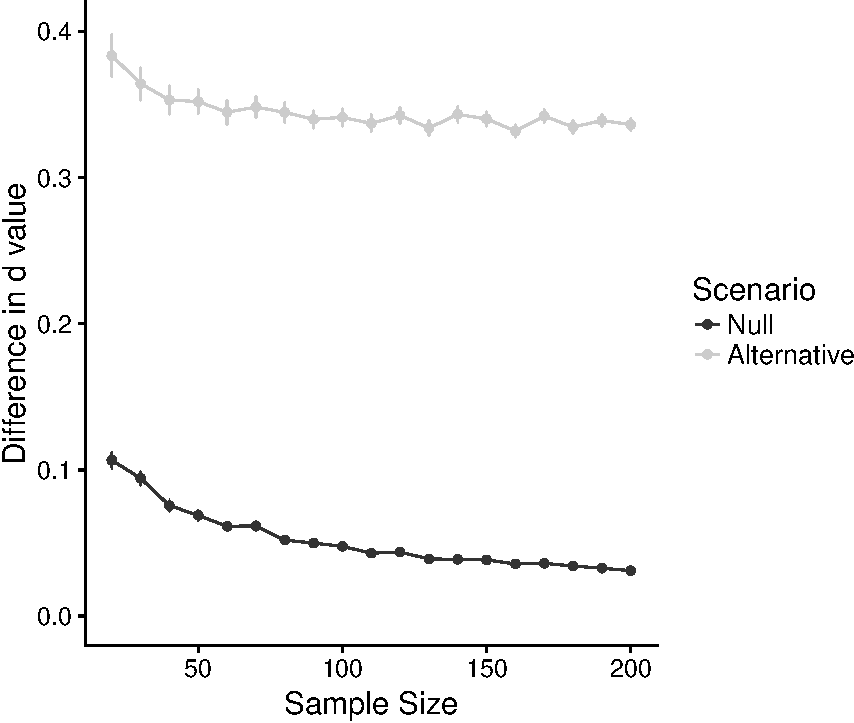
\includegraphics{SAD_manuscript_files/figure-latex/sense-graph-1.pdf}
\caption{\label{fig:sense-graph}Difference in effect size for sensitivity
analysis in null and alternative scenarios across sample size. Error
bars represent 95\% confidence interval of bootstrapped difference
scores.}
\end{figure}

A sensitivity analysis was included in our preregistered plan; however,
no demographic information was collected as part of the survey. To
analyze the effects of low effort and automated data on real analyses,
we created two scenarios sampling from the AMT data: 1) wherein the null
hypothesis was likely and 2) wherein an alternative hypothesis was
likely. These analyses were calculated over a range of sample sizes,
starting at \emph{n} = 20 for each group and increasing in units of 10
until a sample size of \emph{n} = 200 for each group. At each sample
size, 1000 bootstraps were calculated. Within each bootstrapped sample,
a random proportion of flagged data was included in each group. First, a
confidence interval around the proportion of flagged data was calculated
to be .12 to .16. Then, a random proportion was selected from that
range. The selected proportion was used as the sample size proportion
flagged data for each \emph{n} (\emph{p}*\emph{n}), and likewise for
acceptable data for each \emph{n} ((1-\emph{p})*\emph{n}). This process
was used for both groups, resulting in two groups of data, each with a
specific sample size and proportion of flagged data. The dataset sampled
included several missing data points, thus, those scores were dropped
when appropriate.

The total scores were then compared using a \(d_s\) for independent
designs. Second, the flagged data was excluded, and the \(d_s\) values
were calculated again. The data were collected with no experimental
manipulation, and therefore, this simulation was not expected to show
large differences between groups (supporting the null hypothesis). To
simulate the effects of flagged data on an alternative hypothesis, 14
points (i.e., a one point change for each item on the RS-14 scale, thus,
a total of 14-point change) was added to the total score of the
acceptable data only in one of the randomized groupings. This addition
pushed apart the means of the acceptable data, with the assumption that
the flagged data would not show this manipulation. The same \(d_s\)
values were calculated comparing bootstrapped groupings.

To interpret these analyses, the absolute value change in effect sizes
was examined across sample size. The average difference values between
tests with flagged data and tests without are presented in Figure
\ref{fig:sense-graph} across sample size. The results from these
comparisons indicated that flagged data has a small effect when the null
hypothesis was more likely, which decreases across sample size,
\(\Delta d_s\) = 0.05. However, when the alternative hypothesis was more
likely, the effect of flagged data increases wherein \(\Delta d_s\) =
0.34 change in effect size was found, which was more consistent across
values of \emph{n}. This result implies that the inclusion of flagged
data can decrease the power of a statistical test by under-representing
the effect size in the study. The decrease in power can be attributed to
the addition of noise to a study, which increases the standard error,
therefore, decreasing the test statistic. The complete detection
algorithm is provided to researchers on our OSF page and part of a
completely reproducible manuscript in \emph{R} markdown.

\section{Discussion}\label{discussion}

Amazon Mechanical Turk (AMT) is a popular marketplace to collect data
quickly and cheaply, serving as an invaluable tool for researchers with
constrained budgets and time. Hundreds of articles are published
annually utilize AMT, with many being published in high impact academic
journals (Chandler \& Paolacci, 2017). While the quality of data have
been initially questioned, reliability of AMT data has shown to be
sufficient (Goodman et al., 2012; Gosling et al., 2004; Krantz \& Dalal,
2000; Mason \& Suri, 2012; Paolacci et al., 2010; Suri et al., 2011). We
must ensure the data quality of our data samples, as this facet impacts
the reliability of research findings. This type of screening is an
important methodological step in any area of research. For instance, the
process of detecting and excluding outlying and influential cases is
common in statistical analyses. Test statistics, such as \emph{t} and
\emph{F}, focus on optimizing the quality of signal, while attenuating
corresponding statistical noise. Participant screening methods aimed at
identifying low effort responses or potentially automated responses will
ensure that the signal to noise ratio is the best representation of the
phenomena studied.

Multiple checks were employed to differentiate automated, random/low
effort, and high effort responses. Comparisons between these three
conditions were made on the basis of click counts, response latencies,
distribution fit, and skewness and kurtosis. The characteristics from
each condition were then utilized for the development of an adaptable
\emph{R} function to identify potential automated responses, as well as
low effort responses. Identified cases were subsequently used in the
context of a sensitivity analysis to warrant exclusion from statistical
analyses in a sample of AMT participants. Response time has been noted
to follow a power law, leading to difficulties in predicting the
necessary time required to complete certain tasks (Ipeirotis, 2010).
Page response times in the current project were calculated based on
minimum reading speed (Trauzettel-Klosinski \& Dietz, 2012). Given this
difficulty and mixed research regarding the utilization of response time
as a screening method, page submit time was used in conjunction with
other screening methods.

Zhu and Carterette (2010) looked at various patterns of participant
responses and found that low quality or effort responses was linked to
what is referred to as \enquote{low-entropy} patterns of response.
Essentially, this pattern of data is characteristic of participants who
choose a low or minimum number of scale options, for instance switching
back and forth between only two scale options. Considering this finding,
the number of utilized scale options were also used as a criterion.
However, we showed that not all low-effort responses follow this
pattern, as both automated and low effort data were shown to use the
majority of scale options. Depending on a given scale or hypothesis,
researchers might also expect a low-varying range of scale options.
Uniform distribution fit was also more likely to occur with low effort
and automated data compared to high effort data.

Previous literature has noted that the exclusion of participants based
on response time or manipulation checks alone may not be sufficient. We
agree that any one measure by itself is not sufficient to exclude
participants. For instance, when taken alone, the page time submit
identifier identified more than half of participants as problematic. A
more nuanced approach to participant screening is appropriate, analogous
to the multiple diagnostic checks used in general linear models to
examine model assumptions or the presence of outliers and influential
cases. By using multiple indicators, we can more accurately identify low
effort participants. The current project has developed an \emph{R}
function that can be adapted for researchers using surveys as a research
tool. This function is available in the supplementary materials and can
be adapted to various surveys where valuable information is collected,
such as timing and click counts. We suggest the use of participant
screening methods as an adaptive one, based on specific research design,
methodology, and hypotheses. We acknowledge that there may not be a
\enquote{one size fits all} solution. However, by using multiple checks
available at hand, or relevant to specific hypotheses, we can begin a
more transparent process of screening out noise. A straightforward and
practical guideline for researchers collecting data from crowd-sourcing
platforms would be to collect 15 percent more participants than
originally planned, in anticipation of excluding low effort and
automated responses. The relevance of better statistical checks prior to
main analyses extends to many areas, as high quality data is the coin of
the realm in quantitative research.

Appropriate participant screening methods, especially in the case of
online data collection, is integral in psychological science. With a
lack of internal control, researchers must be aware and ensure that the
quality of data being received matches the quality of data expected out
of participants, beyond that of simply reproducing effects typically
found in laboratory settings. Optimizing the signal to noise ratio
through the use of a multiple check participant screening method can be
an invaluable tool to researchers, and can be implemented in tandem to
the normal pipeline of pre-analysis checks, such as checks for missing
data, statistical outliers, and model assumptions. Last, the SAD
screening procedure may be best implemented as part of pre-registered
plan of data screening to best ensure transparency in research process
from data collection to statistical analysis (van't Veer \&
Giner-Sorolla, 2016).

\newpage

\section{References}\label{references}

\setlength{\parindent}{-0.5in} \setlength{\leftskip}{0.5in}

\hypertarget{refs}{}
\hypertarget{ref-Aiena2014}{}
Aiena, B. J., Baczwaski, B. J., Schulenberg, S. E., \& Buchanan, E. M.
(2014). Measuring resilience with the RS14: A tale of two samples.
\emph{Journal of Personality Assessment}, \emph{97}(3), 291--300.
doi:\href{https://doi.org/10.1080/00223891.2014.951445}{10.1080/00223891.2014.951445}

\hypertarget{ref-Berg2006}{}
Berg, G. J. van den, Lindeboom, M., \& Dolton, P. J. (2006). Survey
non-response and the duration of unemployment. \emph{Journal of the
Royal Statistical Society: Series A (Statistics in Society)},
\emph{169}(3), 585--604.
doi:\href{https://doi.org/10.1111/j.1467-985x.2006.00422.x}{10.1111/j.1467-985x.2006.00422.x}

\hypertarget{ref-Berinsky2012}{}
Berinsky, A. J., Huber, G. A., \& Lenz, G. S. (2012). Evaluating online
labor markets for experimental research: Amazon.com's Mechanical Turk.
\emph{Political Analysis}, \emph{20}(3), 351--368.
doi:\href{https://doi.org/10.1093/pan/mpr057}{10.1093/pan/mpr057}

\hypertarget{ref-Buchanan2017}{}
Buchanan, E. M., Valentine, K. D., \& Scofield, J. E. (2017). MOTE.
Retrieved from \url{https://github.com/doomlab/MOTE}

\hypertarget{ref-Buhrmester2011}{}
Buhrmester, M., Kwang, T., \& Gosling, S. D. (2011). Amazon's Mechanical
Turk: A new source of inexpensive, yet high-quality, data?
\emph{Perspectives on Psychological Science}, \emph{6}(1), 3--5.
doi:\href{https://doi.org/10.1177/1745691610393980}{10.1177/1745691610393980}

\hypertarget{ref-Casler2013}{}
Casler, K., Bickel, L., \& Hackett, E. (2013). Separate but equal? A
comparison of participants and data gathered via Amazon's MTurk, social
media, and face-to-face behavioral testing. \emph{Computers in Human
Behavior}, \emph{29}(6), 2156--2160.
doi:\href{https://doi.org/10.1016/j.chb.2013.05.009}{10.1016/j.chb.2013.05.009}

\hypertarget{ref-Chandler2017}{}
Chandler, J. J., \& Paolacci, G. (2017). Lie for a dime: When most
prescreening responses are honest but most study participants are
imposters. \emph{Social Psychological and Personality Science},
194855061769820.
doi:\href{https://doi.org/10.1177/1948550617698203}{10.1177/1948550617698203}

\hypertarget{ref-Cohen1988}{}
Cohen, J. (1988). \emph{Statistical power analysis for the behavioral
sciences} (2nd ed.). Routledge.

\hypertarget{ref-Cumming2013}{}
Cumming, G. (2013). The new statistics. \emph{Psychological Science},
\emph{25}(1), 7--29.
doi:\href{https://doi.org/10.1177/0956797613504966}{10.1177/0956797613504966}

\hypertarget{ref-Downs2010}{}
Downs, J. S., Holbrook, M. B., Sheng, S., \& Cranor, L. F. (2010). Are
your participants gaming the system? Screening Mechanical Turk workers.
\emph{Proceedings of the SIGCHI Conference on Human Factors in Computing
Systems}, 2399--2402.
doi:\href{https://doi.org/10.1145/1753326.1753688}{10.1145/1753326.1753688}

\hypertarget{ref-Felstiner2011}{}
Felstiner, A. (2011). Working the crowd: Employment and labor law in the
crowdsourcing industry. \emph{Berkeley Journal of Employment \& Labor
Law}, \emph{32}(1), 143--204.
doi:\href{https://doi.org/10.15779/Z38Z92X}{10.15779/Z38Z92X}

\hypertarget{ref-Fort2011}{}
Fort, K., Adda, G., \& Cohen, K. B. (2011). Amazon Mechanical Turk: Gold
mine or coal mine? \emph{Computational Linguistics}, \emph{37}(2),
413--420.
doi:\href{https://doi.org/10.1162/COLI_a_00057}{10.1162/COLI\_a\_00057}

\hypertarget{ref-Goodman2012}{}
Goodman, J. K., Cryder, C. E., \& Cheema, A. (2012). Inside the Turk:
Methodological concerns and solutions in Mechanical Turk
experimentation. \emph{Advances in Consumer Research}, \emph{40},
112--117.

\hypertarget{ref-Gosling2004}{}
Gosling, S. D., Vazire, S., Srivastava, S., \& John, O. P. (2004).
Should we trust web-based studies? A comparative analysis of six
preconceptions about internet questionnaires. \emph{American
Psychologist}, \emph{59}(2), 93--104.
doi:\href{https://doi.org/10.1037/0003-066x.59.2.93}{10.1037/0003-066x.59.2.93}

\hypertarget{ref-Henrich2010}{}
Henrich, J., Heine, S. J., \& Norenzayan, A. (2010). The weirdest people
in the world? \emph{Behavioral and Brain Sciences}, \emph{33}(2-3),
61--83.
doi:\href{https://doi.org/10.1017/S0140525X0999152X}{10.1017/S0140525X0999152X}

\hypertarget{ref-Ipeirotis2010}{}
Ipeirotis, P. G. (2010). Analyzing the Amazon Mechanical Turk
marketplace. \emph{The ACM Magazine for Students}, \emph{17}(2), 16--21.
doi:\href{https://doi.org/10.1145/1869086.1869094}{10.1145/1869086.1869094}

\hypertarget{ref-Krantz2000}{}
Krantz, J. H., \& Dalal, R. (2000). Validity of web-based psychological
research. In \emph{Psychological experiments on the internet} (pp.
35--60). Elsevier.
doi:\href{https://doi.org/10.1016/b978-012099980-4/50003-4}{10.1016/b978-012099980-4/50003-4}

\hypertarget{ref-Lakens2013}{}
Lakens, D. (2013). Calculating and reporting effect sizes to facilitate
cumulative science: A practical primer for t-tests and ANOVAs.
\emph{Frontiers in Psychology}, \emph{4}.
doi:\href{https://doi.org/10.3389/fpsyg.2013.00863}{10.3389/fpsyg.2013.00863}

\hypertarget{ref-Lawrence2016}{}
Lawrence, M. A. (2016). \emph{Ez: Easy analysis and visualization of
factorial experiments}. Retrieved from
\url{https://CRAN.R-project.org/package=ez}

\hypertarget{ref-Mason2012}{}
Mason, W. A., \& Suri, S. (2012). Conducting behavioral research on
Amazon's Mechanical Turk. \emph{Behavior Research Methods},
\emph{44}(1), 1--23.
doi:\href{https://doi.org/10.3758/s13428-011-0124-6}{10.3758/s13428-011-0124-6}

\hypertarget{ref-Olejnik2003}{}
Olejnik, S., \& Algina, J. (2003). Generalized eta and omega squared
statistics: measures of effect size for some common research designs.
\emph{Psychological Methods}, \emph{8}(4), 434--447.
doi:\href{https://doi.org/10.1037/1082-989X.8.4.434}{10.1037/1082-989X.8.4.434}

\hypertarget{ref-Paolacci2014}{}
Paolacci, G., \& Chandler, J. J. (2014). Inside the Turk. \emph{Current
Directions in Psychological Science}, \emph{23}(3), 184--188.
doi:\href{https://doi.org/10.1177/0963721414531598}{10.1177/0963721414531598}

\hypertarget{ref-Paolacci2010}{}
Paolacci, G., Chandler, J. J., \& Ipeirotis, P. G. (2010). Running
experiments on Amazon Mechanical Turk. \emph{Judgment and Decision
Making}, \emph{5}(5), 411--419.
doi:\href{https://doi.org/10.2139/ssrn.1626226}{10.2139/ssrn.1626226}

\hypertarget{ref-Sorokin2008}{}
Sorokin, A., \& Forsyth, D. (2008). Utility data annotaton with Amazon
Mechanical Turk. \emph{Proceedings of the 1st IEEE Workshop on Internet
Vision at CVPR 08}, (c), 1--8.
doi:\href{https://doi.org/10.1109/CVPRW.2008.4562953}{10.1109/CVPRW.2008.4562953}

\hypertarget{ref-Stieger2010}{}
Stieger, S., \& Reips, U.-D. (2010). What are participants doing while
filling in an online questionnaire: A paradata collection tool and an
empirical study. \emph{Computers in Human Behavior}, \emph{26}(6),
1488--1495.
doi:\href{https://doi.org/10.1016/j.chb.2010.05.013}{10.1016/j.chb.2010.05.013}

\hypertarget{ref-Suri2011}{}
Suri, S., Goldstein, D. G., \& Mason, W. A. (2011). Honesty in an online
labor market. In \emph{Paper presented at the 3rd Association for the
Advancement of Artificial Intelligence Human Computation Workshop}. San
Francisco, CA.

\hypertarget{ref-Trauzettel-Klosinski2012}{}
Trauzettel-Klosinski, S., \& Dietz, K. (2012). Standardized assessment
of reading performance: The new international reading speed texts IReST.
\emph{Investigative Ophthalmology and Visual Science}, \emph{53}(9),
5452--5461.
doi:\href{https://doi.org/10.1167/iovs.11-8284}{10.1167/iovs.11-8284}

\hypertarget{ref-VantVeer2016}{}
van't Veer, A. E., \& Giner-Sorolla, R. (2016). Pre-registration in
social psychology---A discussion and suggested template. \emph{Journal
of Experimental Social Psychology}, \emph{67}, 2--12.
doi:\href{https://doi.org/10.1016/j.jesp.2016.03.004}{10.1016/j.jesp.2016.03.004}

\hypertarget{ref-Wagnild2009}{}
Wagnild, G. M. (2009). A review of the Resilience Scale. \emph{Journal
of Nursing Measurement}, \emph{17}(2), 105--113.
doi:\href{https://doi.org/10.1891/1061-3749.17.2.105}{10.1891/1061-3749.17.2.105}

\hypertarget{ref-Wagnild1993}{}
Wagnild, G. M., \& Young, H. M. (1993). Development and psychometric
evaluation of the Resilience Scale. \emph{Journal of Nursing
Measurement}, \emph{1}(2), 165--178.

\hypertarget{ref-Zhu2010}{}
Zhu, D., \& Carterette, B. (2010). An analysis of assessor behavior in
crowdsourced preference judgments. In \emph{In M. Lease, V. Carvalho, \&
E. Yilmaz (Eds.), Proceedings of the ACM SIGIR 2010 Workshop on
Crowdsourcing for Search Evaluation}. Geneva, Switzerland.






\end{document}
